\documentclass{article}
\usepackage{tikz}
\usetikzlibrary{arrows.meta}

\begin{document}

\begin{figure}[h]
    \centering
    \begin{tikzpicture}[scale=0.8, every node/.style={scale=0.8}]
        % Draw the memory addresses
        \foreach \x/\y in {0/0x0, 10/0x10, 20/0x20, 40/0x40} {
            \draw[->, thick] (\x, 1) -- ++(0,-1) node[below] {\y};
        }
        
        % Draw the ALock structure
        \draw[thick] (0, -1) rectangle (3, 0);
        \draw[thick] (3, -1) rectangle (6, 0);
        \draw[thick] (6, -1) rectangle (9, 0);
        
        % Label the fields
        \node at (1.5, -0.5) {$tail_r$};
        \node at (4.5, -0.5) {$tail_l$};
        \node at (7.5, -0.5) {victim};
        
        % Draw the alignment line
        \draw[decorate, decoration={brace, amplitude=10pt}, thick] (0, -1) -- (9, -1) node[midway, below=10pt] {64B};
    \end{tikzpicture}
    
    \caption{64B-aligned ALock containing 8B pointers to the remote and local cohort tails, and an integer victim field to indicate the current victim cohort. Values are padded to the address alignments shown.}
\end{figure}

\end{document}